%& C:\Users\Sam\AppData\Roaming\TikzEdt\TikzEdt\023~1.0\TEMP_H~1
\begin{document}
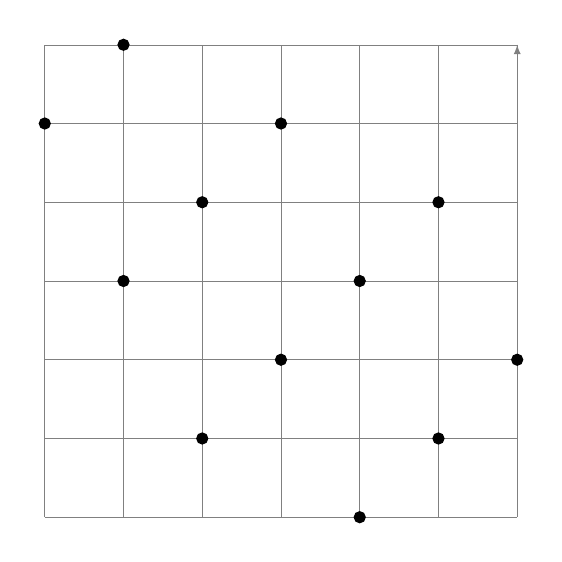
\begin{tikzpicture}


\node (v12) at (2,1) {};
\node (v13) at (3,-1) {};
\node (v15) at (0,2) {};
\node (v16) at (-2,3) {};
\node (v14) at (1,0) {};
\node (v17) at (2,-2) {};
\node (v18) at (-1,1) {};
\node (v19) at (0,-1) {};
\node (v20) at (1,-3) {};
\node (v21) at (-1,-2) {};
\node (v22) at (-2,0) {};
\node (v23) at (-3,2) {};
\draw [-latex][help lines, step=1cm] (-3,-3) grid (3,3);

\draw [fill]
(v12) circle (2pt)
(v13) circle (2pt)
(v14) circle (2pt)
(v15) circle (2pt)
(v16) circle (2pt)
(v17) circle (2pt)
(v18) circle (2pt)
(v19) circle (2pt)
(v20) circle (2pt)
(v21) circle (2pt)
(v22) circle (2pt)
(v23) circle (2pt)
;


\usetikzlibrary{calc}
\pgftransformreset
\node[inner sep=0pt,outer sep=0pt,minimum size=0pt,line width=0pt,text width=0pt,text height=0pt] at (current bounding box) {};
%add border to avoid cropping by pdflibnet
\foreach \border in {0.1}
  \useasboundingbox (current bounding box.south west)+(-\border,-\border) rectangle (current bounding box.north east)+(\border,\border);
\newwrite\metadatafile
\immediate\openout\metadatafile=\jobname_BB.txt
\path
  let
    \p1=(current bounding box.south west),
    \p2=(current bounding box.north east)
  in
  node[inner sep=0pt,outer sep=0pt,minimum size=0pt,line width=0pt,text width=0pt,text height=0pt,draw=white] at (current bounding box) {
\immediate\write\metadatafile{\p1,\p2}
};
\immediate\closeout\metadatafile
\end{tikzpicture}

\end{document}
